\documentclass[aps,pra,twocolumn,amsmath,amssymb,nofootinbib,superscriptaddress]{revtex4}

\newcommand{\bra}[1]{\langle#1|}
\newcommand{\ket}[1]{|#1\rangle}
\newcommand{\op}[2]{\hat{\textbf{#1}}_{#2}}
\newcommand{\dagop}[2]{\hat{\textbf{#1}}_{#2}^\dag}
\newcommand{\keith}[1]{{\color{cyan}{#1}}}
\newcommand{\peter}[1]{{\color{blue}{#1}}}
\newcommand{\remove}[1]{{\color{red}{#1}}}

\usepackage[pdftex]{graphicx}
\usepackage{mathrsfs}
\usepackage[colorlinks]{hyperref}

\begin{document}

\bibliographystyle{apsrev}

%
% Title
%

\title{An introduction to boson-sampling}

%
% Authors
%

\author{In no particular order}

\author{Peter P. Rohde}
\email[]{dr.rohde@gmail.com}
\homepage{http://www.peterrohde.org}
\affiliation{Centre for Engineered Quantum Systems, Department of Physics and Astronomy, Macquarie University, Sydney NSW 2113, Australia}

\author{Bryan Gard}

\author{Keith R. Motes}

\author{Jonathan P. Dowling}

\date{\today}

\frenchspacing

%
% Abstract
%

\begin{abstract}
\end{abstract}

\maketitle

\section{Introduction (Bryan)}

\subsection{Motivation for LOQC and boson-sampling (Bryan)}

\section{Intro to LOQC (Bryan)}

\section{Why is LOQC hard? (Bryan)}

\section{The boson-sampling formalism}

Unlike full LOQC, which requires active elements, the boson-sampling model is strictly passive, requiring only single-photon sources, passive linear optics (i.e beamsplitters and phase-shifters), and photodetection. No quantum memory or feedforward is required.

We begin by preparing an input state comprising $n$ single photons in $m$ modes,
\begin{eqnarray} \label{eq:input_state}
\ket{\psi_\mathrm{in}} &=& \ket{1_1,\dots,1_n,0_{n+1},\dots,0_m} \nonumber \\
&=& \hat{a}^\dag_1 \dots \hat{a}^\dag_n \ket{0_1,\dots,0_m},
\end{eqnarray}
where $\hat{a}^\dag_i$ is the photon creation operator in the $i$th mode. It is assumed that the number of modes scales quadratically with the number of photons, \mbox{$m=O(n^2)$}. The input state is evolved via a passive linear optics network, which implements a unitary map on the creation operators,
\begin{equation}
\hat{U}\hat{a}_i^\dag\hat{U}^\dag = \sum_{j=1}^m U_{i,j} \hat{a}_j^\dag,
\end{equation}
where $U$ is a unitary matrix characterising the linear optics network. It was shown by Reck \emph{et al.} \cite{bib:Reck94} that any $U$ may be efficiently decomposed into $O(m^2)$ optical elements. The output state is a superposition of the different configurations of how the $n$ photons could have arrived in the output modes,
\begin{equation}
\ket{\psi_\mathrm{out}} = \sum_S \gamma_S \ket{n_1^{(S)},\dots,n_m^{(S)}},
\end{equation}
where $S$ is a configuration, $n_i^{(S)}$ is the number of photons in the $i$th mode associated with configuration $S$, and $\gamma_S$ is the amplitude associated with configuration $S$. The probability of measuring configuration $S$ is given by \mbox{$P_S = |\gamma_S|^2$}. The full model is illustrated in Fig.~\ref{fig:model}

\begin{figure}[!htb]
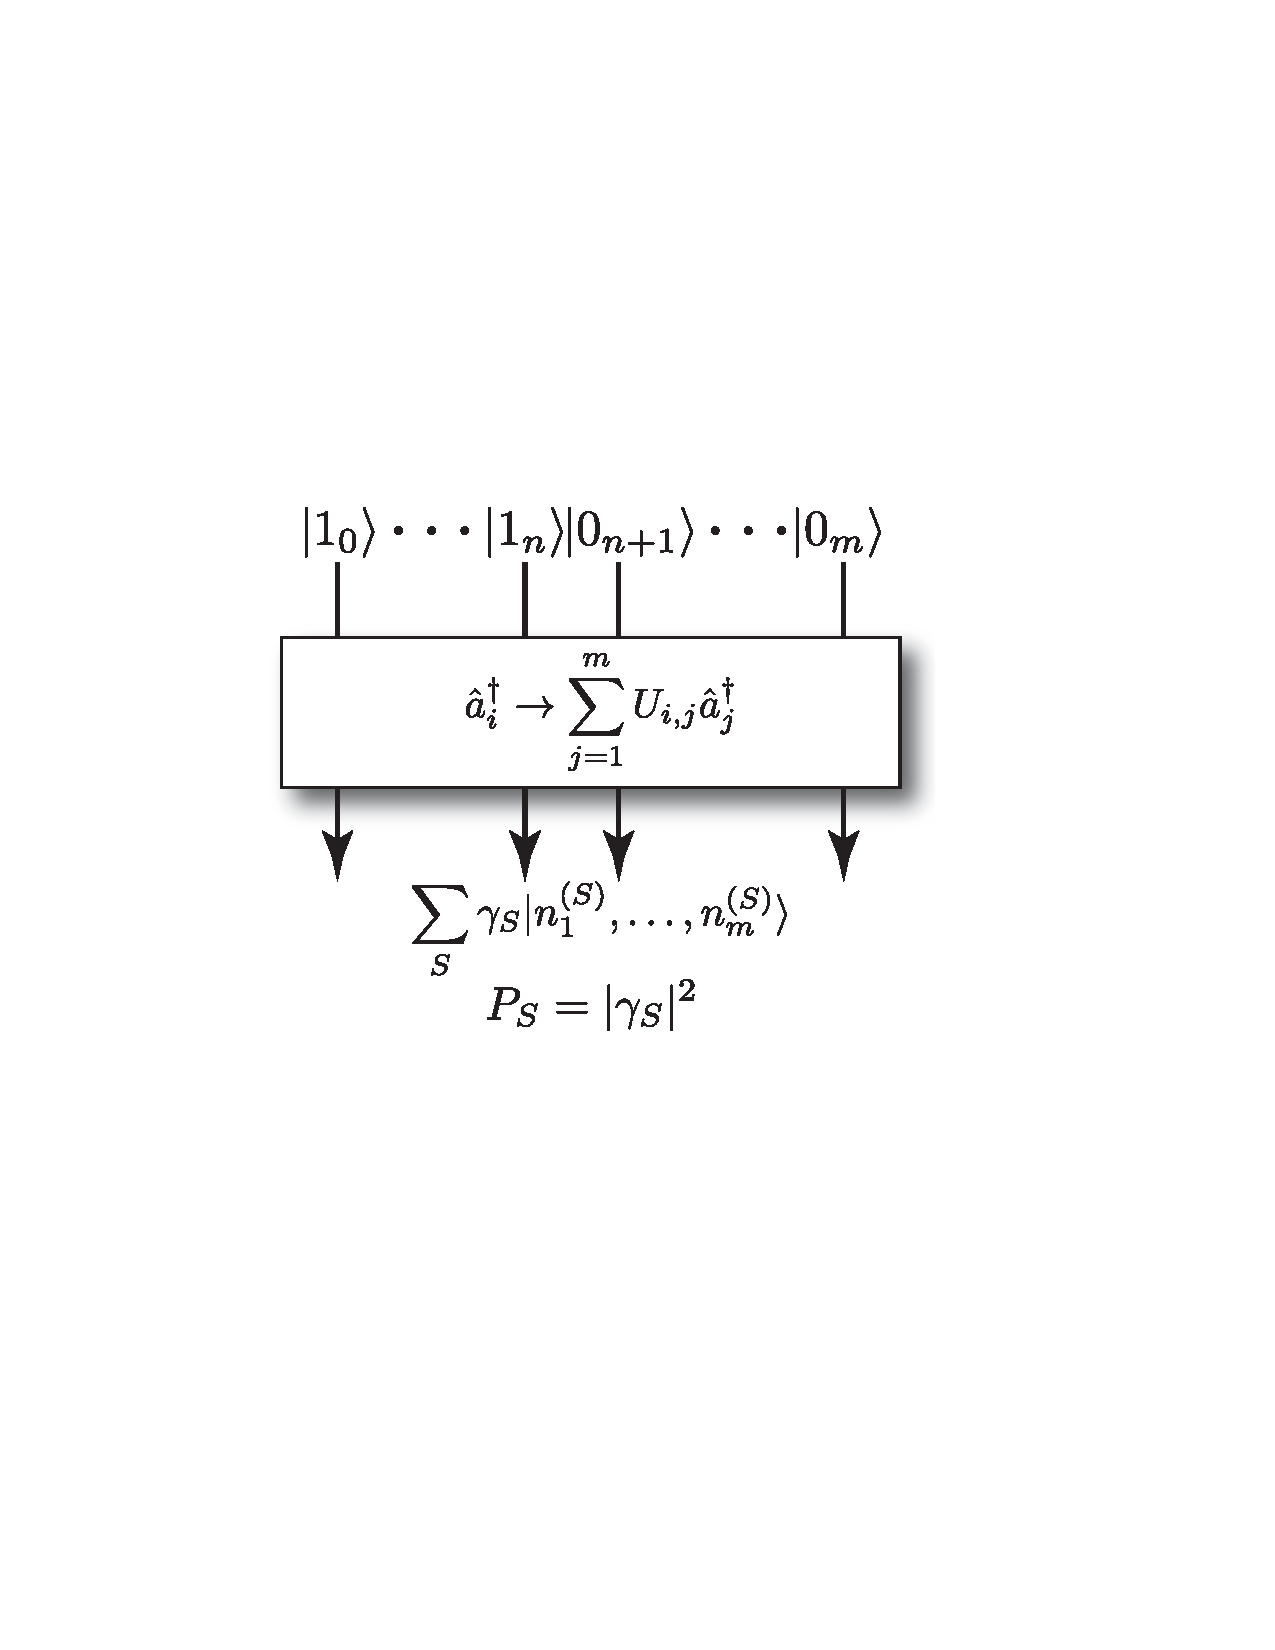
\includegraphics[width=0.7\columnwidth]{model}
\caption{The boson-sampling model. $n$ single photons are prepared in $m$ optical modes. These are evolved via a passive linear optics network $\hat{U}$. Finally the ouput statistics are sampled via concidence photodetection. The experiment is repeated many times, reconstructing the output distribution $P_S$.} \label{fig:model}
\end{figure}

It was shown by Scheel \cite{bib:Scheel04perm} that the amplitudes $\gamma_S$ are related to matrix permanents,
\begin{equation}
\gamma_S = \frac{\mathrm{Per}(U_S)}{\sqrt{s_1!\dots s_m!}},
\end{equation}
where $s_i$ is the number of photons in the $i$th output mode of configuration $S$, $U_S$ is an \mbox{$n\times n$} sub-matrix of $U$, and \mbox{$\mathrm{Per}(U_S)$} is the permanent of $U_S$.

Let us examine this relationship with the permanent more closely. Consider Fig.~\ref{fig:two_photon_perm}. Here the first two modes have single photons, with the remaining modes in the vacuum state. Let us consider the amplitude of measuring one photon at output mode 2 and another at output mode 3. Then there are two ways in which this could occur. Either the first first reaches mode 2 and the second mode 3, or vice versa, i.e the photons pass straight through, or swap. Therefore there are $2!=2$ ways in which the photons could reach the outputs. Thus, this amplitude may be written as,
\begin{eqnarray} \label{eq:coinProbEx}
\gamma_{\{2,3\}} &=& \underbrace{U_{1,2}U_{2,3}}_{\mathrm{walkers\ don't\ swap}} + \underbrace{U_{1,3}U_{2,2}}_{\mathrm{walkers\ swap}} \nonumber \\
&=& \mathrm{Per} \left[ {\begin{array}{cc}
   U_{1,2} & U_{2,2} \\
   U_{1,3} & U_{2,3} \\
  \end{array} } \right],
\end{eqnarray}
which is a \mbox{$2\times 2$} matrix permanent.

\begin{figure}[!htb]
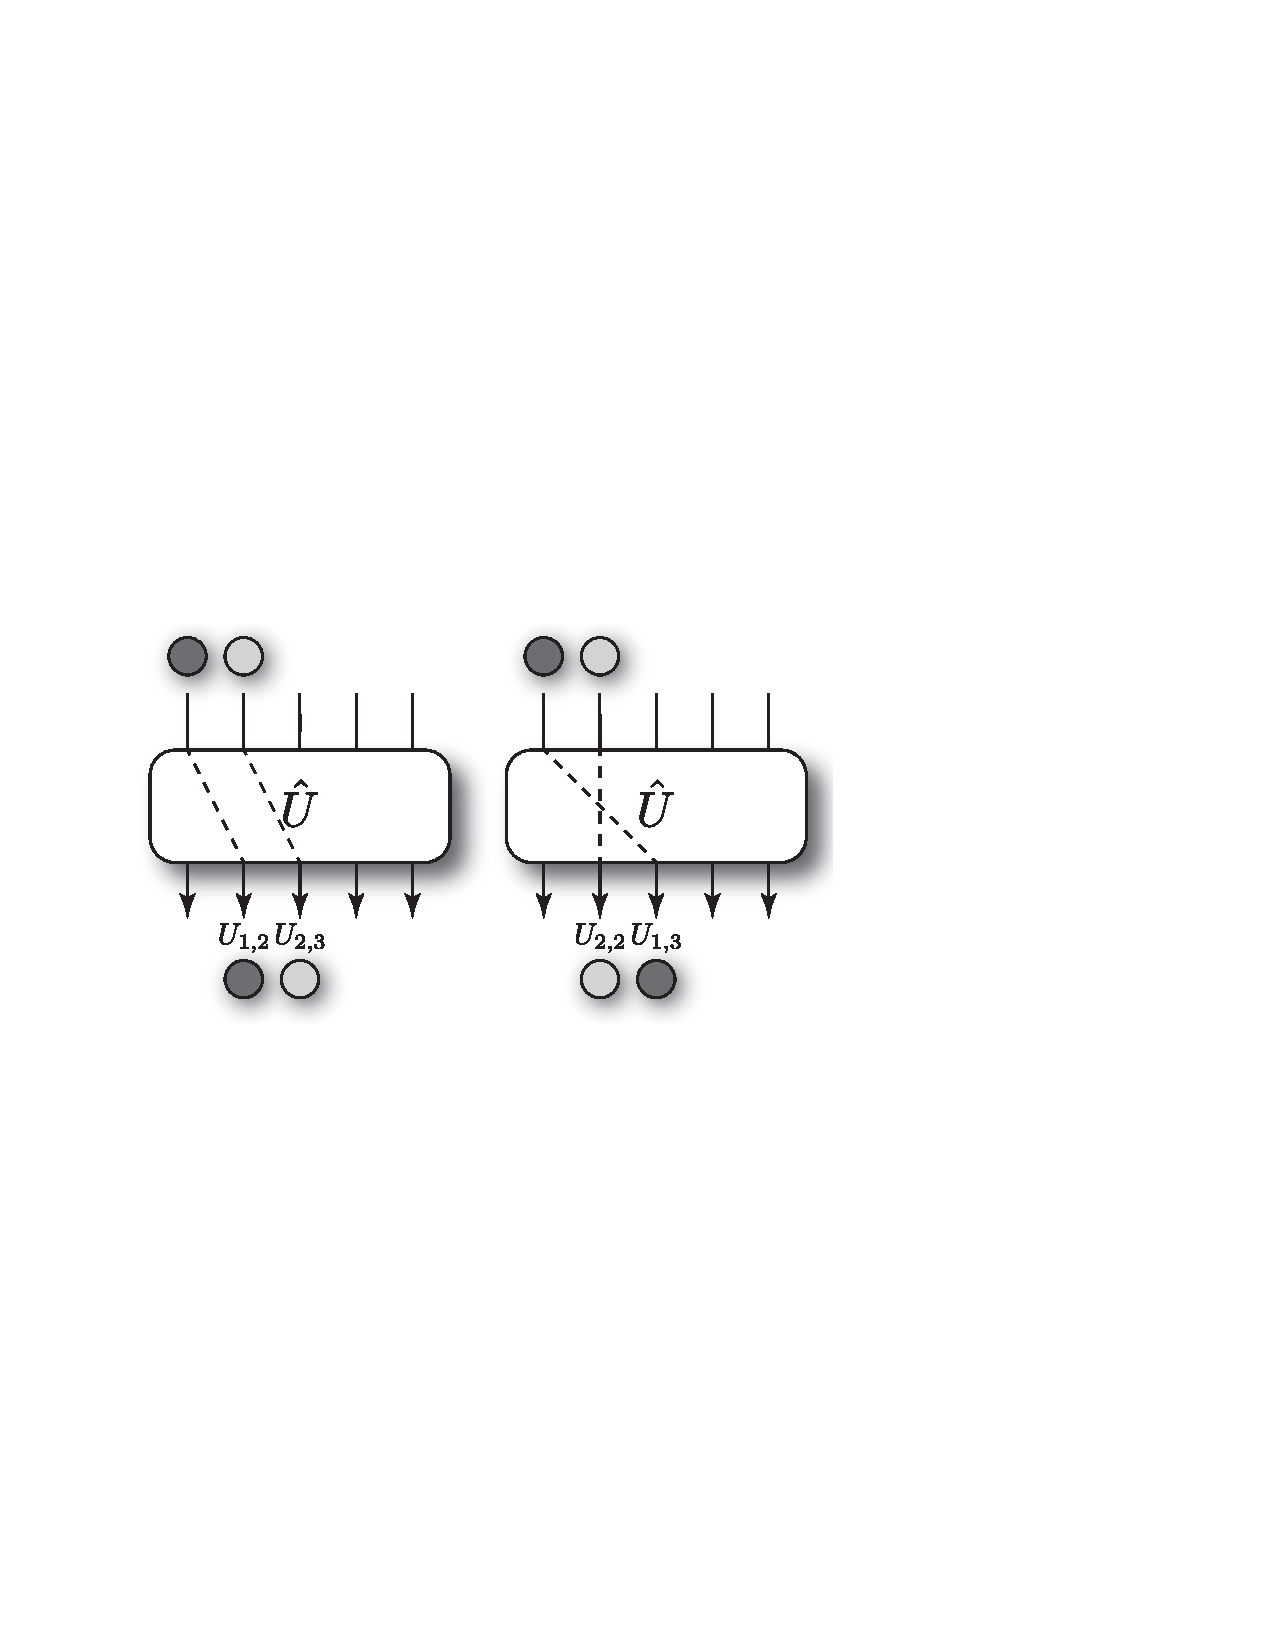
\includegraphics[width=0.7\columnwidth]{two_photon_combinatorics}
\caption{Two-photon boson-sampling, where we wish to calculate the amplitude of measuring a photon at each of the output modes 2 and 3. There are two ways in which this may occur -- either the photons pass straight through, or swap, yielding a sum of two paths.} \label{fig:two_photon_perm}
\end{figure}

As a slightly more complex example, consider the three photon case shown in Fig.~\ref{fig:three_photon_perm}. Now we see that there are \mbox{$3!=6$} ways in which the three photons could reach the outputs, and the associated amplitude is given by a \mbox{$3\times 3$} matrix permanent,
\begin{eqnarray} \label{eq:coinProbEx3}
\gamma_{\{1,2,3\}} &=& U_{1,1}U_{2,2}U_{3,3} + U_{1,1}U_{3,2}U_{2,3} \nonumber \\
&+& U_{2,1}U_{1,2}U_{3,3} + U_{2,1}U_{3,2}U_{1,3} \nonumber \\
&+& U_{3,1}U_{1,2}U_{2,3} + U_{3,1}U_{2,2}U_{1,3}
\nonumber \\
&=& \mathrm{Per} \left[ {\begin{array}{ccc}
   U_{1,1} & U_{2,1} & U_{3,1} \\
   U_{1,2} & U_{2,2} & U_{3,2} \\
   U_{1,3} & U_{2,3} & U_{3,3} \\
  \end{array} } \right].
\end{eqnarray}

\begin{figure}[!htb]
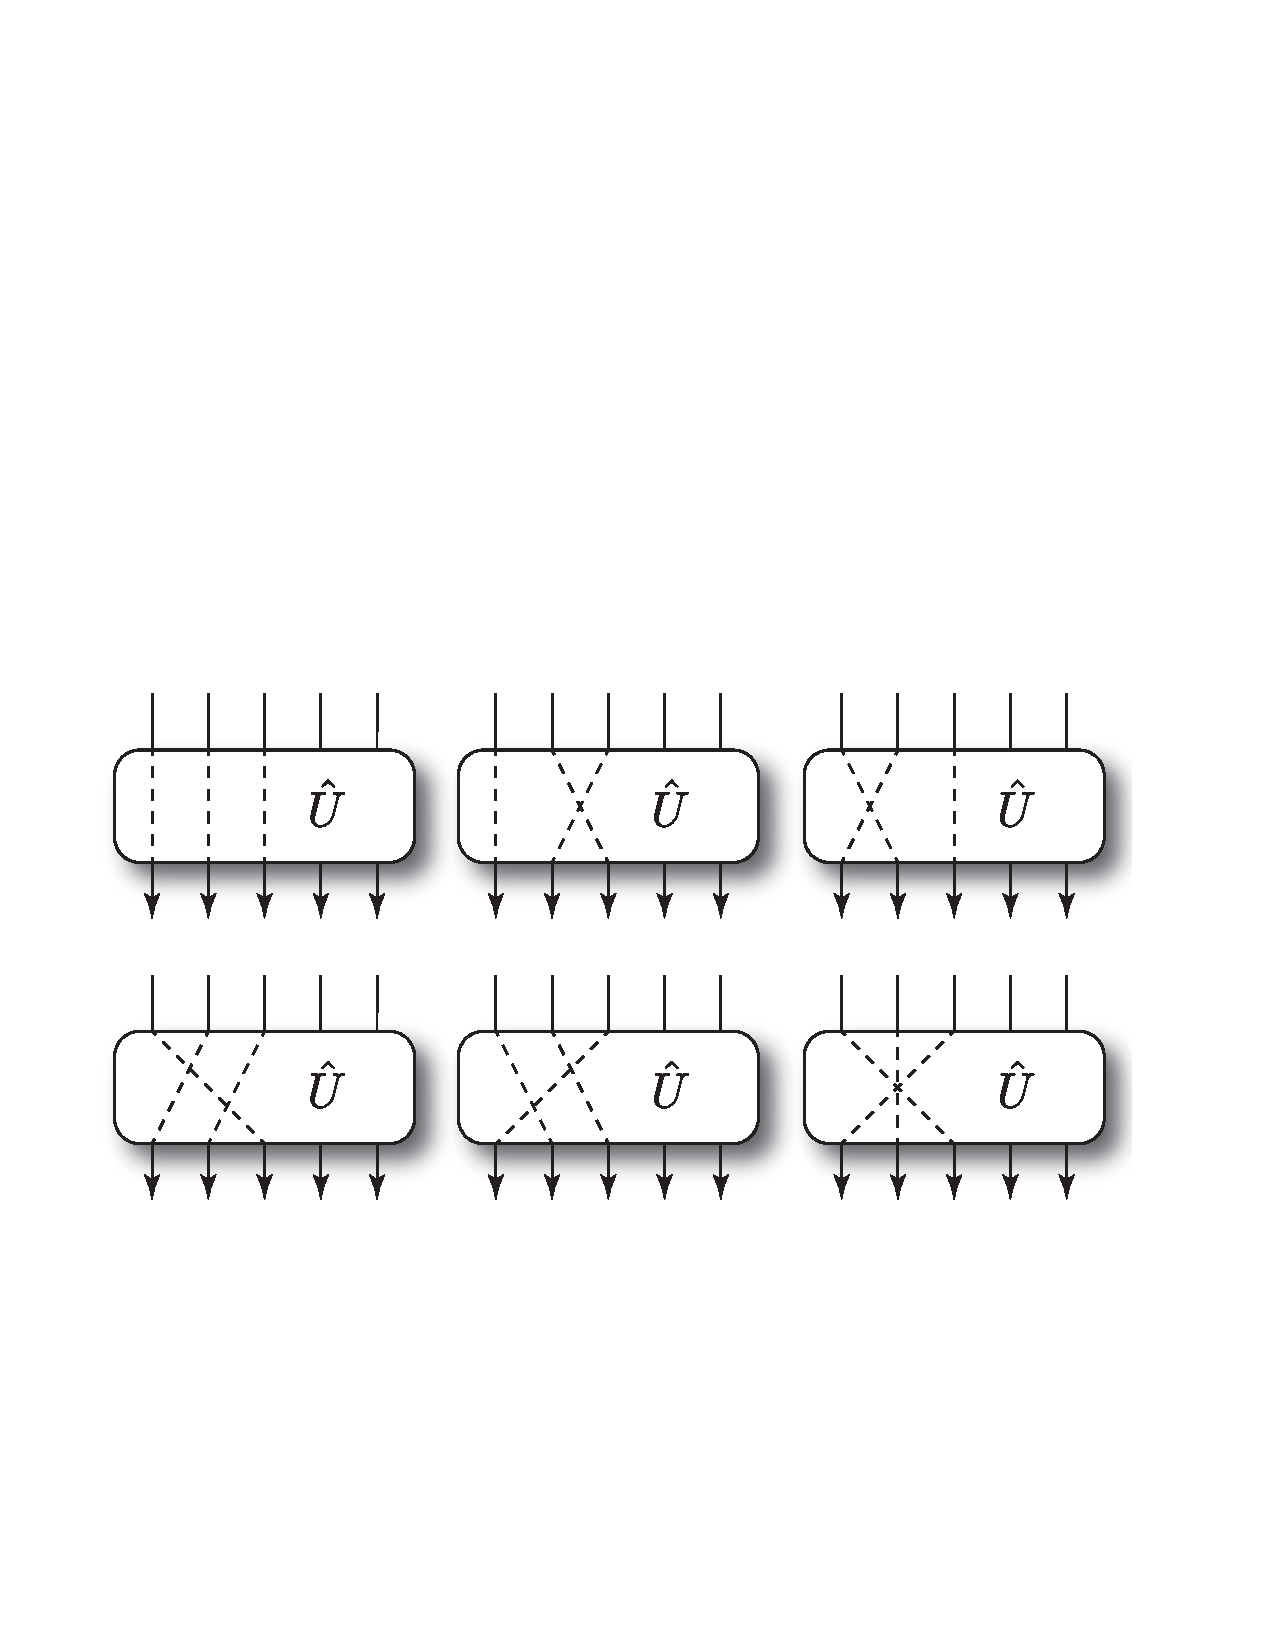
\includegraphics[width=\columnwidth]{three_photon_combinatorics}
\caption{Thee photon boson-sampling, where we wish to calculate the amplitude of measuring a photon at each of the output modes 1, 2 and 3. There are now \mbox{$3!=6$} possible routes for this to occur.} \label{fig:three_photon_perm}
\end{figure}

In general, with $n$ photons, there will be $n!$ ways in which the photons could reach the outputs (assuming they all arrive at distinct outputs), and the associated amplitude will relate to an \mbox{$n\times n$} matrix permanent. The best known algorithm for calculating matrix permanents is by Ryser \cite{bib:Ryser63}, whose algorithm requires \mbox{$O(2^n n^2)$} runtime. Thus, we can immediately see that if boson-sampling were to be classically simulated by calculating the matrix permanents, it would require exponential classical resources.

Because the number of modes scales quadratically with the number of photons, for large systems we are statistically gauranteed that all photons will arrive at different output modes. This implies that in this regime on/off (or `bucket') detectors will suffice, and photon-number resolution is not necessary, a further experimental simplification compared to full-fledged LOQC.

The number of configurations in the output modes scales as,
\begin{equation}
|S| = \binom{n+m-1}{n},
\end{equation}
which is exponential is $n$. Thus, with an `efficient' (i.e sub-exponential) number of trials, we are unlikely to sample from a given configuration more than once. This implies that we are unable to determine any given $P_S$ with more than binary accuracy. Thus, boson-sampling does \emph{not} let us \emph{calculate} matrix permanents, as doing so would require determining amplitudes with a high level of precision, which would require an exponential number of measurements.

The experiment is repeated may times, each time performing a coincidence photodetection at the output modes. Thus, after each run we sample from the distribution $P_S$. This yields a so-called \emph{sampling problem}, whereby the goal is to sample a statistical distribution using a finite number of measurements. This is in contrast to well-known \emph{decision problems}, such as Shor's algorithm \cite{bib:Shor97}, which provide a well-defined answer to a well-posed question.

This sampling problem was shown by Aaronson \& Arkhipov to be a computationally hard problem. That is, reconstructing the statistical distribution at the ouput to the boson-sampling device is computationally hard. However, whilst shown to be computationally hard, no known applications for boson-sampling have been described. Thus, boson-sampling acts as an interesting proof-of-principle demonstration that linear optics can outperform classical computers, but, based on present understanding, does not solve a problem of practical interest.

\subsection{Sampling problems vs. decision problems (Peter)}

\subsection{Why is boson-sampling so much easier than linear optics quantum computing? (Peter)}

\subsection{Errors in boson-sampling (Johnny)}
Discuss the 1/poly(n) bound

\section{Boson-sampling and the Extended Church-Turing thesis}

Any model for quantum computation is subject to errors of some form. In the conventional circuit model, this includes error such as dephasing. In linear optics, this includes photon loss and mode-mismatch. Let us consider a very generic error model for boson-sampling, where the single photon states are the desired single photon with probability $p$, otherwise are in some erroneous state \cite{bib:BSECT}. This erroneous state could, for example, comprise terms with the wrong photon number (such as loss or second order excitations), or mode-mismatch. Then our input state is of the form,
\begin{equation}
\hat\rho_\mathrm{in} =\left(\bigotimes_{i=1}^n[p\ket{1}\bra{1} + (1-p)\hat\rho_\mathrm{error}^{(i)}]\right) \otimes [\ket{0}\bra{0}]^{\otimes^{m-n}},
\end{equation}
where \mbox{$\hat\rho_\mathrm{error}^{(i)}$} may be different for each input mode $i$. This is an independent error model, whereby each state is independently subject to an error channel. $p$ stipulates the fidelity of the single photon states. When \mbox{$p=1$}, the states are perfect single photons, and when \mbox{$p<1$}, the state contain erroneous terms. We desire to sample from the distribution of Eq.~\ref{eq:input_state}, whereby none of the input states are erroneous. This occurs with probability $p^n$.

Let $P$ be the probability that upon performing boson-sampling we have sampled from the correct distribution, otherwise we sample from noise. The complexity proof provided by Aaronson \& Arkhipov only considered the regime where \mbox{$P>1/\mathrm{poly}(n)$}. Thus, for computational hardness, we require \mbox{$p^n > 1/\mathrm{poly}(n)$}. Clearly in the asymptotic limit of large $n$, this bound can never be satisified for any $p<1$. Thus, with this independent error model, boson-sampling will always fail in the asymptotic limit.

Numerous authors \cite{bib:Broome20122012, bib:ShenDuan13, bib:AA13response, bib:Shchesnovich13, bib:Molmer13} have claimed that large-scale demonstrations of boson-sampling could provide elucidation on the Extended Church-Turing (ECT) thesis -- the statemenent that any physical system may be efficiently simulated on a Turing machine. However, it must be noted that the ECT thesis is by definition an asymptotic statement about arbitrarily large systems. Because the required error bound for boson-sampling is never satisfied in this limit, it is clear that boson-sampling cannot elucidate the validitiy of the ECT thesis as asymptotically large boson-sampling devices must fail under an independent error model.

This concern might be overcome in the future with either (1) a loosing of the error bound to $1/\mathrm{exp}(n)$, or (2) the development of fault-tolerance techniques for boson-sampling. However, to-date no such developments have been made. Thus, based on \emph{present} understanding, boson-sampling will not answer the question as to whether the ECT thesis is correct or not. However, this is distinct from the question `will boson-sampling yield \emph{post-classical} computation?'. The answer to this question may very well be affirmative, as this only requires a finite sized device, just big enough to beat the best classical computers.

\section{Boson-sampling with other classes of quantum optical states (Johnny)}

\section{How to build a boson-sampling device (Keith)}

In this section we explain the basic components required to build a linear optical boson-sampling device. This device consists of three basic components which are single-photon sources, linear optical networks, and photon detectors each having their own issues to overcome, which are described below. Also, there are multiple options for each component and thus multiple ways of building a boson-sampling device. Although boson-sampling is much easier to implement than full scale LOQC it remains  challenging to build a post-classical boson-sampling machine. 

\subsection{Photon sources (Keith)}

\textbf{add in citations}

Optical boson-sampling begins by preparing $n$ single photon Fock states to create the input state $\ket{\Psi_{\mathrm{in}}}=\ket{1,1,\dots,1,0,0,\dots,0}$. This state can be generated using various types of available photon sources. For a review of many of the photon-sources see \cite{bib:SourceAndDetectorReview}. The most common is spontaneous parametric down conversion (SPDC), which are used in most linear optical experiments involving single-photons. 

The SPDC source works by first pumping a non-linear crystal with a laser source. With some probability one of the laser photons interacts with the crystal and emits an entangled superposition of photons along two paths. The photons in one path are called the signal photons and the photons in the other path are called the idler photons. The signal photons are measured by a photo-detector and with a successful click we know that the idler photons exist. The idler photons are then routed into one of the input ports of the boson-sampling device. The output state of the SPDC source is,
\begin{equation} \label{SPDC}
\ket{\Psi_{SPDC}} = \sqrt{1-\chi^2}\sum_{n=0}^{\infty}\chi^n\ket{n}_s\ket{n}_i,
\end{equation}
where $\chi$ is the squeezing parameter, $n$ is the number of photons, $s$ represents the signal photons, and $i$ represents the idler photons. For boson-sampling we would ideally like the SPDC source to output only the single-photon term $\ket{1}_s\ket{1}_i$.  

There are several problems associated with SPDC sources which limit the scalability of boson-sampling. The major problem is higher order photon terms. In the boson-sampling model we only want the $\ket{1}_s\ket{1}_i$ term which is far from deterministic using SPDC sources. For instance, the SPDC source is going to emit the zero photon term with highest probability. Also, photon terms of larger than one will emit with exponentially decreasing probability. Now if we let the probability of successfully emitting the single photon terms with an SPDC source be $\eta$, then we can characterise the error rates. Since boson-sampling requires $n$ photons and the error associated with each SPDC source is $1-\eta$, then the total error due to unprobabilistic photon emissions scale as $(1-\eta)^{n}$, which is exponential in $n$. It was shown by Aaronson \& Arkhipov that boson-sampling can only tolerate polynomial error scaling rate with $n$, so this totally kills the boson-sampling device.

One way to get around this error with SPDC sources is to consider a multiplexing device \cite{bib:migdall2002tailoring}. There has been recent experimental progress in developing active multiplexing devices \cite{bib:LPOR201400027, bib:ma2011experimental}. It was recently shown my Motes \emph{et al.} that SPDC sources are scalable in the asymptotic limit for boson-sampling \cite{bib:motes2013spontaneous}. The boson-sampling architecture with multiplexing is shown and described in Fig.\ref{fig:multiplexing}. 

\begin{figure}[!htb]
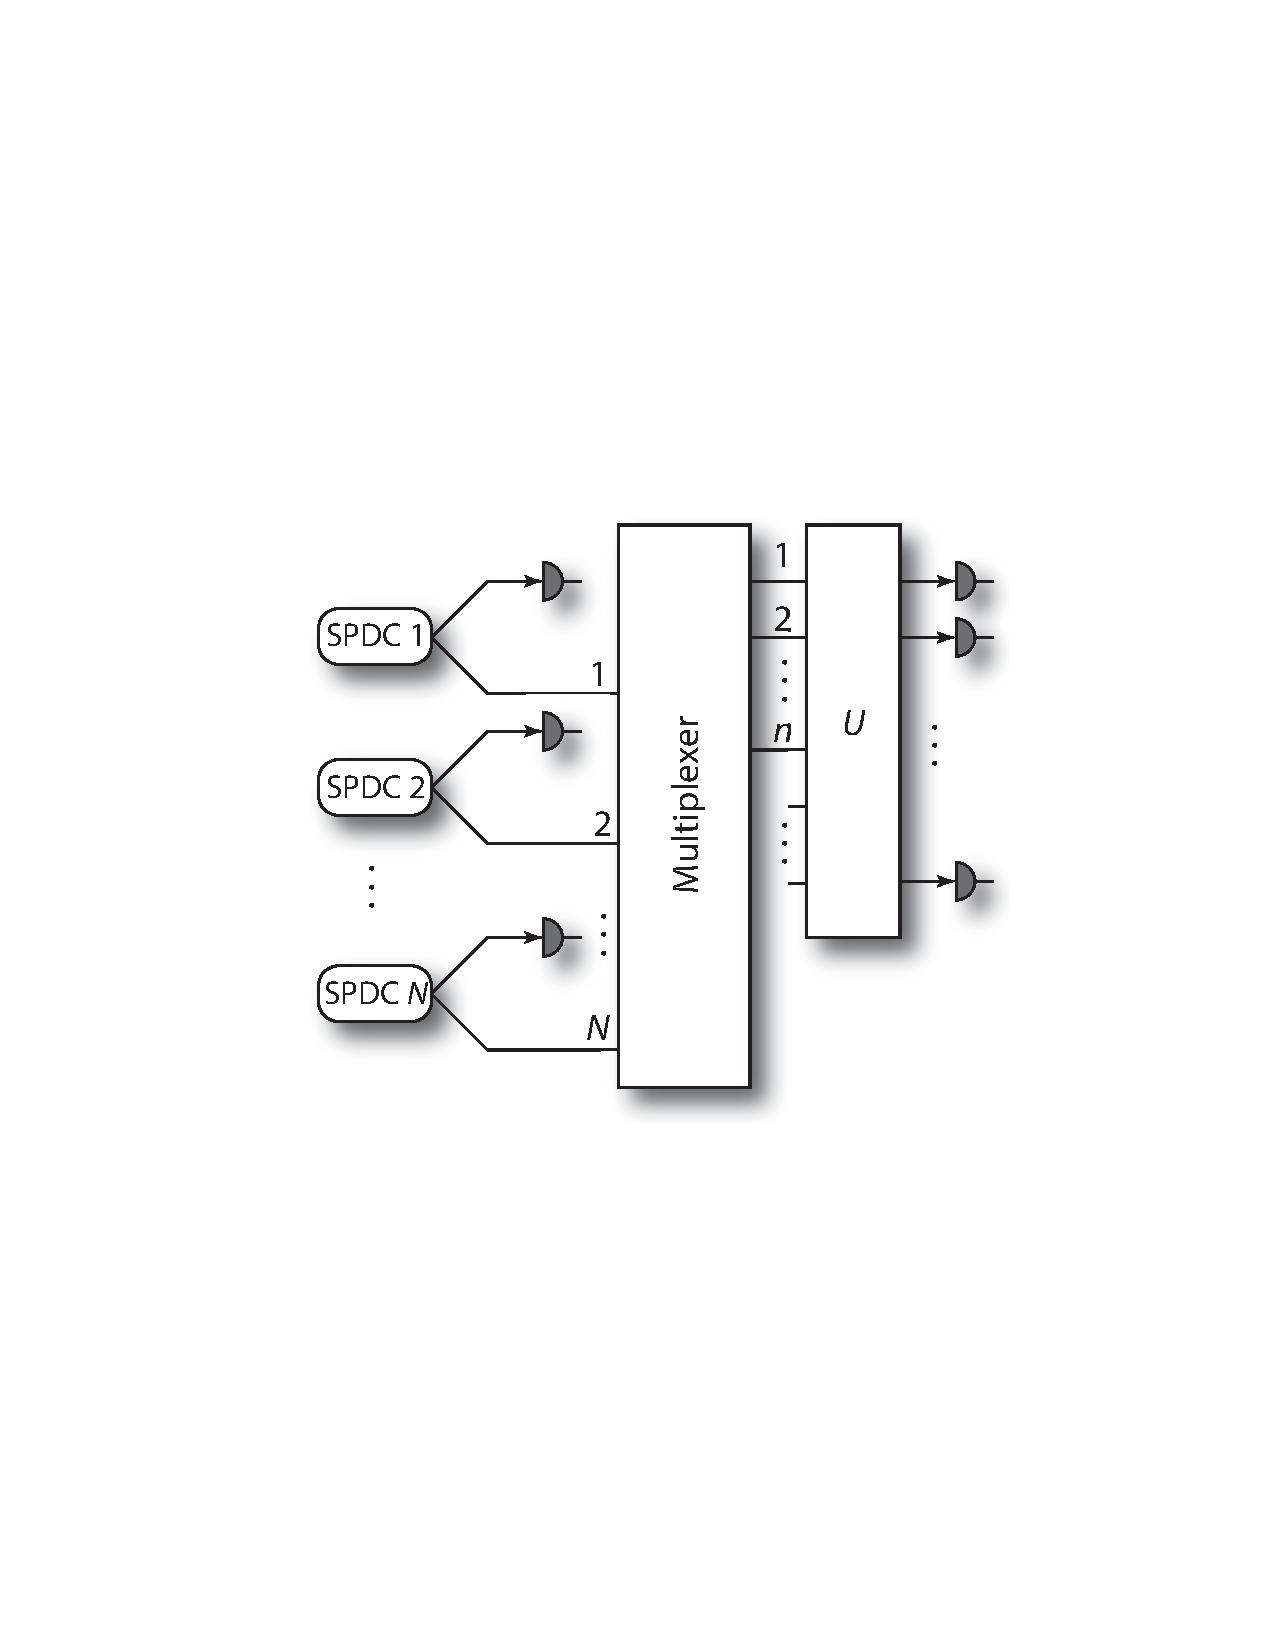
\includegraphics[width=0.7\columnwidth]{multiplexing}
\caption{Boson-sampling architecture using SPDC sources with an active multiplexer. $N$ sources operate in parallel, each heralded by an inefficient single-photon number-resolving detector. It is assumed that \mbox{$N\gg n$}, which guarantees that at least $n$ photons will be heralded. The multiplexer dynamically routes the successfully heralded modes to the first $n$ modes of the unitary network $U$. Finally, photodetection is performed and the output is post-selected on the detection on all $n$ photons.}
\label{fig:multiplexing}
\end{figure}

Another problem is that photons from SPDC sources have uncertainty in their temporal distribution. If a boson-sampling device is built using multiple SPDC sources it is difficult to temporally align each of the $n$ photons going into the device. The error term associated with this also scales exponentially with $n$, which as described previously totally renders your boson-sampling device useless. 

\subsection{Linear optical networks (Keith)}
After the input state has been prepared it then passes through some linear optical network denoted by $U$. $U$ transforms the input state as per Eq. \ref{eq:} and may be completely characterized before the experiment using coherent state inputs \cite{bib:PhysRevLett.73.58}. $U$ is composed of an array of discrete elements, namely, beam-splitters and phase shifters.  A beamsplitter and phase shifter can be combined and represented in the following general form \cite{bib:GerryKnight05},
\begin{equation} \label{eq:BS}
U_{\mathrm{BS}}(t) = \left( \begin{array}{cc}
e^{i(\alpha-\frac{\beta}{2}-\frac{\gamma}{2})}\mathrm{cos}\left(\frac{\delta}{2}\right) & -e^{i(\alpha-\frac{\beta}{2}+\frac{\gamma}{2})}\mathrm{sin}\left(\frac{\delta}{2}\right)  \\
e^{i(\alpha+\frac{\beta}{2}-\frac{\gamma}{2})}\mathrm{sin}\left(\frac{\delta}{2}\right) & e^{i(\alpha+\frac{\beta}{2}+\frac{\gamma}{2})}\mathrm{cos}\left(\frac{\delta}{2}\right)
\end{array} \right), 
\end{equation}
where $0\leq\alpha\leq2\pi$ and $0\leq\{\beta,\gamma,\delta\}\leq\pi$ are arbitrary phases. It was shown by Reck \emph{et al.} that an arbitrary unitary transformation $U$ can be constructed with  $O(m^2)$ optical elements \cite{bib:PhysRevLett.73.58}, where $m$ is the number of inputs to the boson-sampling device. 

For a $U$ that would implement a classically hard problem one would need hundreds of optical elements. Constructing an arbitrary $U$ using the traditional linear optical approach of setting and aligning each optical element would be quite tedious if not impossible. This approach would also occupy the space and resources of entire optical labs, which is unfeasible. Thus, the traditional approach is quite impracticable and is a major problem with boson-sampling; however, there are potential routes to avoid some of these issues.  

One method to simplify the linear optical network is to use integrated waveguides. Quantum interference was first demonstrated with this technology by Peruzzo \emph{et al.} \cite{bib:peruzzo2011multimode}. Also, this technology promises superior performance, scalability, and miniaturization by integrating the linear optical network onto a chip \cite{bib:Politi02052008, bib:matthews2009, bib:Politi04092009}. Aligning would no longer be a major problem as the waveguide would be laser written using computers. The waveguide can have hundreds of modes on a relatively small silicon chip \cite{}, so space is no longer a major issue. The main issue with integrated waveguides is achieving sufficiently low loss rates inside of the waveguide and in the coupling of the waveguide to the photon-sources and photo-detectors. The current lose rates in these waveguides are too high and post-selection upon $n$ photons at the output would almost never happen. It is possible that the photon-sources and photo-detectors however will eventually be built into the waveguide which would greatly reduce the loss.   

Another potential route to simplifying the linear optical network is to use time-bin encoding in a loop based architecture \cite{bib:motes2014scalable}. The major advantage of this architecture is that it only requires two delay loops, two on/ off switches, and one controllable phase shifter as shown and described in Fig. \ref{fig:fiber_loop}. This possibility eliminates the problem of aligning hundreds of optical elements and it eliminates the size problem because it can be set up on a small optics table. A major problem with this architecture however is that it remains difficult to control a dynamic phase-shifter with high fidelity at a rate that is on the order of the time-bin width $\tau$.

\begin{figure}[!htb]
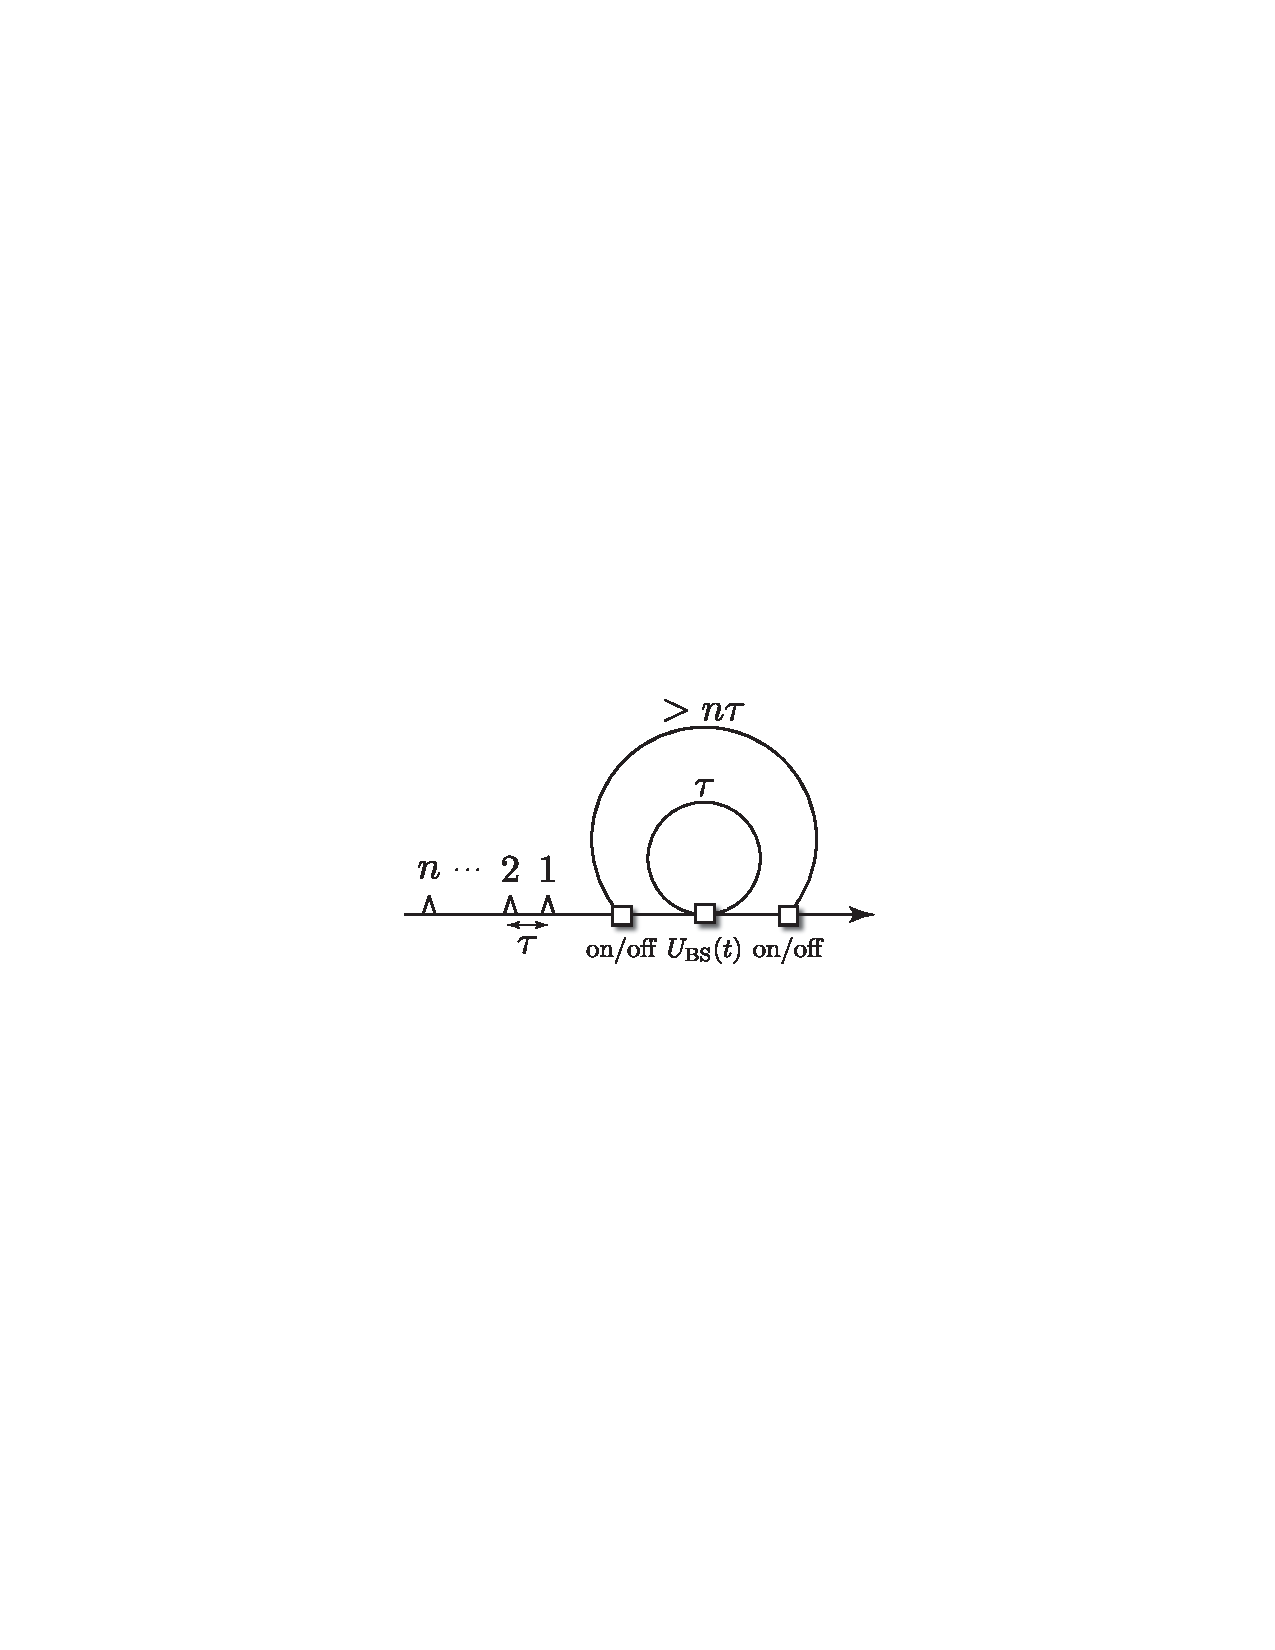
\includegraphics[width=0.7\columnwidth]{fiber_loop}
\caption{The full time-bin encoding architecture for implementing a boson-sampling device. Single photons arrive in a train of time-bins instead of in spatial modes. Each time-bin corresponds to spatial modes in the boson-sampling scheme and are separated by time $\tau$. The photon train gets coupled completely in by the first switch. The photons then transverse the inner loop such that each time-bin may interact. The first (last) photon is coupled completely in (out) so that input and output time-bins match. The outer loop allows an arbitrary number of the smaller loops to be applied consecutively which is determined by the third switch. Finally, the photon train is measured at the output and regular boson-sampling statistics apply. Note that any delay line will work in this architecture.}
\label{fig:fiber_loop}
\end{figure}

\subsection{Photo-detection (Keith)}
The final task of the boson-sampling device is sampling the output distribution. With linear optical boson-sampling this is done with photo-detectors. For a review on many of the various photo-detectors see \cite{bib:SourceAndDetectorReview}.  

There are two general types of photo-detectors -- photon-number resolving detectors and bucket detectors. The former counts the number of photons that are absorbed by the detector. These are much more difficult to make and more expensive in general than bucket detectors. Bucket detectors simply fire if there are photons present or don't fire if there are no photons present. It does not inform the user of the number of photons that entered the detector. Detection of a single photon is notoriously difficult with all sorts of possible errors occurring. Some of these errors include the detector measuring extraneous photons which is called dark counting, it could count two photons when there was one and vice versa, and it could trigger when there were no photons present, among others.

In boson-sampling the number of input and output modes scale as $O(n^2)$. In other words there is an order of magnitude more modes than photons. This is to avoid the bosonic birthday paradox where photons would tend to bunch in the same output mode. When large amounts of bunching occurs the output statistics are classically easy to simulate. This $O(n^2)$ mode scaling is also advantageous for the photo-detection segment of boson-sampling because on average only one photon will arrive in any given output port. Thus, bucket detectors are sufficient for boson-sampling given that the output sample is post-selected upon detecting all $n$ photons. However, if photon-number resolving detectors were used then the samples where multiple photons arrive in the same output mode could be kept. This would be advantageous for sampling distributions that were on the edge of being classically easy and classically difficult to simulate because of more bunching (explain this sentence better). 

Some of the various types of photo-detectors are:

Number-resolving:

Bucket:


\begin{itemize}
\item List different types of detectors
\item don't need to be number resolving.
\item be sure to describe issues to overcome
\end{itemize}

\section{Conclusion (Jon)}

%
% Acknowledgments
%

\begin{acknowledgments}
This research was conducted by the Australian Research Council Centre of Excellence for Engineered Quantum Systems (Project number CE110001013).
\end{acknowledgments}

%
% Bibliography
%

\bibliography{bibliography}

\end{document}
